% Компіляція: lualatex -shell-escape main.tex (двічі)
\documentclass[12pt,a4paper]{article}

\usepackage{fontspec}
\usepackage{polyglossia}
\setdefaultlanguage{ukrainian}
\setmainfont{NewComputerModern10}
\setsansfont{Noto Sans}
\setmonofont{Noto Sans Mono}[Scale=0.82]
\usepackage{amsmath,amssymb,array,booktabs,caption,enumitem,float,geometry,
  graphicx,longtable,microtype,pdflscape,titlesec,xcolor}
\geometry{left=2cm,right=2cm,top=2cm,bottom=2cm}
\setlength{\parindent}{1.25cm}
\setlength{\parskip}{0pt}
\linespread{1.08}
\titleformat{\section}{\normalfont\fontsize{14}{16}\selectfont\bfseries}
  {\thesection}{0.6em}{}
\titleformat{\subsection}{\normalfont\fontsize{12}{14}\selectfont\bfseries}
  {\thesubsection}{0.6em}{}
\captionsetup{font=small,labelfont=bf,labelsep=endash}
\captionsetup[table]{position=bottom,skip=5pt}

\usepackage[newfloat]{minted}
\SetupFloatingEnvironment{listing}{name=Лістинг}
\setminted{fontsize=\scriptsize,linenos,breaklines,breakanywhere,frame=single,
  framesep=2mm,bgcolor=gray!5,tabsize=4}

\usepackage{tikz}
\usetikzlibrary{arrows.meta,shapes.geometric,positioning,calc,fit}
\usepackage[unicode,colorlinks=true,linkcolor=black,urlcolor=blue,
  pdftitle={ІО-41 Давидчук А. М. Лабораторна робота №4},
  pdfauthor={Давидчук Артем Миколайович},
  pdfsubject={OpenMP. Бар’єри, критичні секції. Варіант 7}]{hyperref}

\newcommand{\studentName}{Давидчук А. М.}
\newcommand{\studentGroup}{ІО-41}
\newcommand{\recordBook}{4106}
\newcommand{\teacherName}{Корочкін О. В.}
\newcommand{\reportYear}{2026}
\newcommand{\J}[1]{J_{#1}}

\begin{document}
\pagenumbering{gobble}
\begin{titlepage}
  \begin{center}
    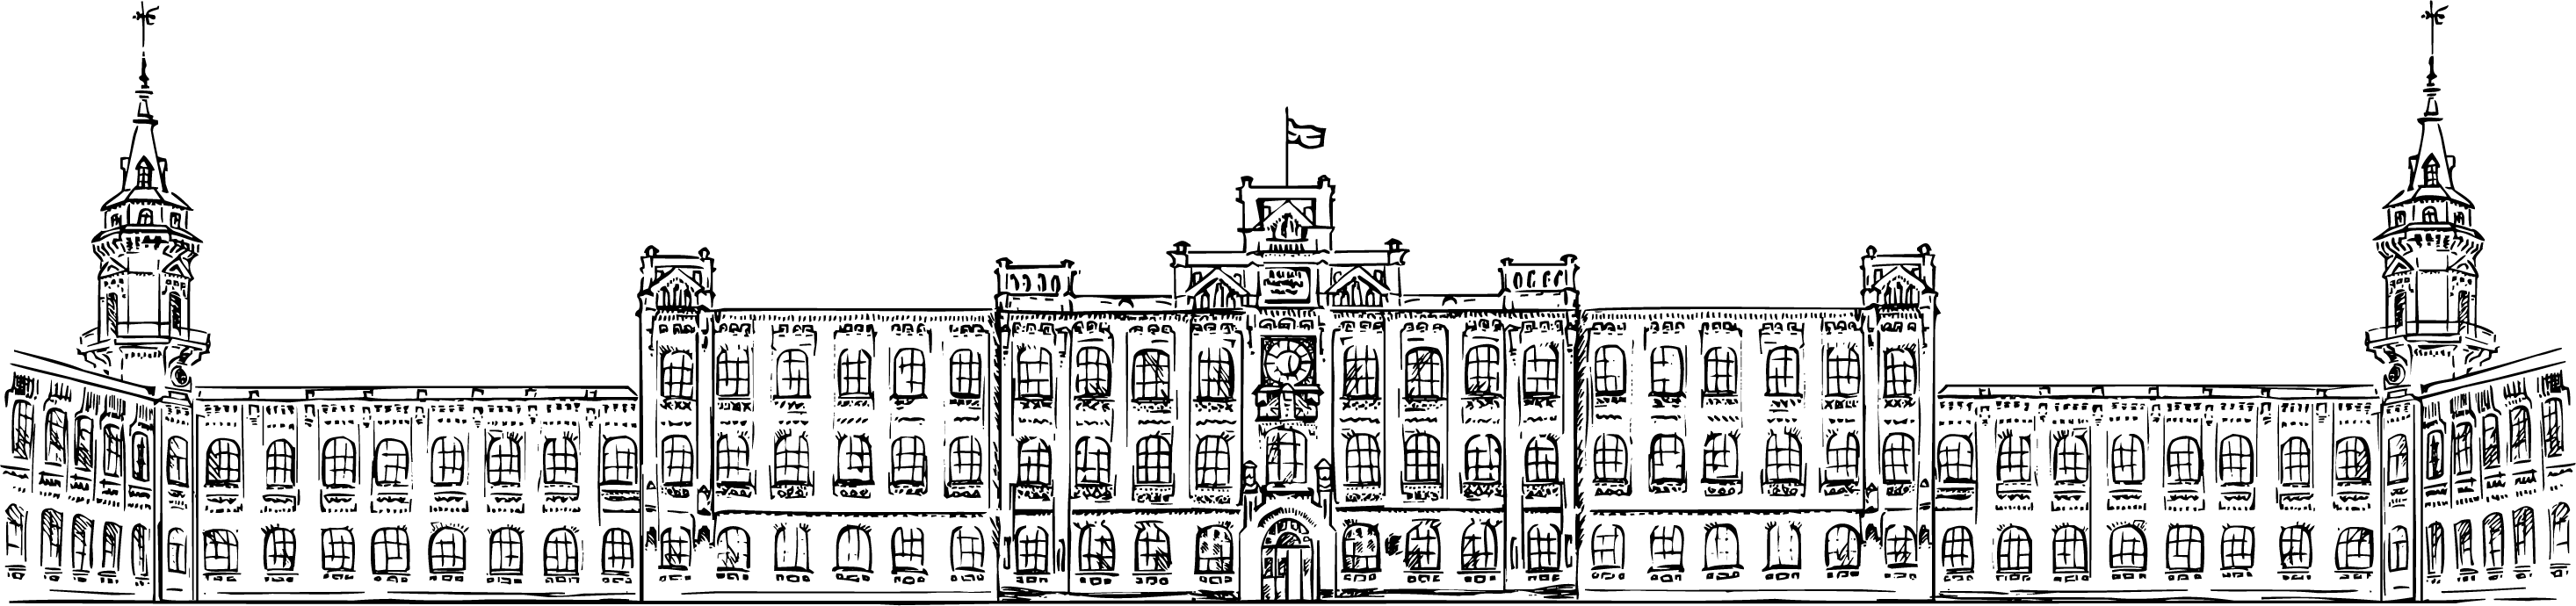
\includegraphics[width=0.7\textwidth]{../../../../../../templates/letterhead.png}
  \end{center}
  \begin{center}\large
    Національний технічний університет України\\
    «Київський політехнічний інститут імені Ігоря Сікорського»\\[1em]
    Факультет інформатики та обчислювальної техніки\\
    Кафедра обчислювальної техніки
  \end{center}
  \vfill
  \begin{center}
    \textbf{\LARGE Паралельні та розподілені обчислення}\\[2em]
    \textbf{\Large Лабораторна робота №4}\\[0.7em]
    \textbf{«Бібліотека OpenMP. Бар’єри, критичні секції»}
  \end{center}
  \vfill
  \begin{flushright}
    \begin{minipage}{0.48\textwidth}
      Виконав: студент 3 курсу ФІОТ,\\
      групи \studentGroup\\
      \textit{\studentName}\\
      Залікова книжка № \recordBook\\
      Варіант завдання: 7\\[1em]
      Перевірив: \textit{\teacherName}
    \end{minipage}
  \end{flushright}
  \vfill
  \begin{center}Київ --- \reportYear\end{center}
\end{titlepage}

\pagenumbering{arabic}
\section{Тема та мета роботи}
\noindent\textbf{Тема:} програмування чотирипроцесорної системи зі спільною
пам’яттю засобами бібліотеки OpenMP.

\medskip
\noindent\textbf{Мета:} розробити паралельний алгоритм обчислення
матричного виразу; організувати роботу чотирьох потоків директивами OpenMP;
реалізувати фазову синхронізацію бар’єрами та взаємне виключення засобами
\texttt{atomic}, \texttt{critical} і \texttt{omp\_lock\_t}; перевірити
правильність і дослідити прискорення програми.

\section{Завдання}
За варіантом 7 необхідно обчислити
\begin{equation}
 MA=(MR\cdot MC)d+(B\cdot Z)(MZ\cdot MM)p.
 \label{eq:task}
\end{equation}
Тут $B,Z$ --- вектори довжини $N$; $MC,MM,MR,MZ,MA$ --- квадратні
матриці порядку $N$; $d,p$ --- скаляри; $B\cdot Z$ --- скалярний добуток.
Кількість потоків $P=4$. Розподіл введення та виведення наведено в
табл.~\ref{tab:io}.

\begin{table}[H]
\centering\renewcommand{\arraystretch}{1.15}
\begin{tabular}{|c|c|c|}\hline
\textbf{Потік}&\textbf{Введення}&\textbf{Виведення}\\\hline
$T_1$&$MC,B$&---\\\hline
$T_2$&$Z,d,p$&---\\\hline
$T_3$&$MM$&$MA$\\\hline
$T_4$&$MR,MZ$&---\\\hline
\end{tabular}
\caption{Розподіл введення і виведення для варіанта 7}
\label{tab:io}
\end{table}

\section{ВИКОНАННЯ ЛР}
\subsection{Етап 1. Розроблення паралельного математичного алгоритму}

Уведемо проміжні матриці та скаляр:
\begin{equation}
 X=MR\cdot MC,\qquad Y=MZ\cdot MM,\qquad s=B\cdot Z.
 \label{eq:intermediate}
\end{equation}
Тоді
\begin{equation}
 MA=dX+spY.
 \label{eq:result}
\end{equation}

Для потоку $T_{t+1}$, $t\in\{0,1,2,3\}$, визначимо діапазон стовпців
\begin{equation}
 a_t=\left\lfloor\frac{tN}{4}\right\rfloor,\qquad
 b_t=\left\lfloor\frac{(t+1)N}{4}\right\rfloor,\qquad
 \J{t}=\{a_t,\ldots,b_t-1\}.
 \label{eq:ranges}
\end{equation}
Діапазони не перетинаються і покривають усі індекси навіть тоді, коли $N$
не кратне чотирьом.

Паралельний алгоритм:
\begin{align}
 X_{i,j}&=\sum_{k=0}^{N-1}MR_{i,k}MC_{k,j},& j&\in\J{t},\label{eq:x}\\
 Y_{i,j}&=\sum_{k=0}^{N-1}MZ_{i,k}MM_{k,j},& j&\in\J{t},\label{eq:y}\\
 s_{t+1}&=\sum_{j=a_t}^{b_t-1}B_jZ_j,\label{eq:si}\\
 s&=s+s_{t+1},\qquad s_{\text{поч}}=0,\label{eq:s}\\
 MA_{i,j}&=dX_{i,j}+spY_{i,j},& j&\in\J{t}.\label{eq:ma}
\end{align}

\subsubsection*{Спільні ресурси}
Вхідні дані після першого бар’єра лише читаються. Потоки записують
неперетинні стовпці $X$, $Y$ і $MA$, тому для цих записів взаємне
виключення не потрібне. Спільним змінюваним ресурсом є накопичувач $s$ у
формулі~\eqref{eq:s}. Перед формулою~\eqref{eq:ma} кожний потік копіює
$s$, $d$ і $p$ у локальні змінні.

\subsection{Етап 2. Розроблення алгоритмів потоків}

Позначення $S_{i,k}$ означає сигнал від $T_i$ про завершення фази $k$,
$W_{i,k}$ --- очікування відповідного сигналу. У реалізації сукупності
сигналів і очікувань однієї фази замінені колективними бар’єрами
$B_1$--$B_3$.

\newcommand{\algtable}[7]{%
\begin{table}[H]\centering\footnotesize\renewcommand{\arraystretch}{1.12}
\begin{tabular}{|c|p{9.7cm}|p{3.25cm}|}\hline
\textbf{№}&\textbf{Алгоритм потоку $#1$}&\textbf{Точка / КД}\\\hline
1&Ввести #2.&КД введення не потрібна: масиви різні\\\hline
2&Сигналізувати завершення введення; чекати введення інших потоків.&$B_1$; #3\\\hline
3&Обчислити стовпці $X_{*,#4}$ за формулою~\eqref{eq:x}.&---\\\hline
4&Обчислити стовпці $Y_{*,#4}$ за формулою~\eqref{eq:y}.&---\\\hline
5&Обчислити локальний скаляр $s_{#5}$ за формулою~\eqref{eq:si}.&---\\\hline
6&Виконати $s=s+s_{#5}$.&КД$_1$: \texttt{atomic}\\\hline
7&Сигналізувати готовність проміжних результатів і чекати решту.&$B_2$; #6\\\hline
8&Скопіювати $s$, $d$, $p$ у локальні змінні.&КД$_2$: lock; КД$_3$, КД$_4$: critical\\\hline
9&Обчислити стовпці $MA_{*,#4}$ за формулою~\eqref{eq:ma}.&---\\\hline
10&Сигналізувати завершення своєї частини $MA$; чекати решту.&$B_3$; #7\\\hline
\end{tabular}\caption{Алгоритм потоку $#1$}\end{table}}

\algtable{T_1}{$MC,B$}{$S_{1,1}$; $W_{2,1},W_{3,1},W_{4,1}$}{\J{0}}{1}
  {$S_{1,2}$; $W_{2,2},W_{3,2},W_{4,2}$}
  {$S_{1,3}$; $W_{2,3},W_{3,3},W_{4,3}$}
\algtable{T_2}{$Z,d,p$}{$S_{2,1}$; $W_{1,1},W_{3,1},W_{4,1}$}{\J{1}}{2}
  {$S_{2,2}$; $W_{1,2},W_{3,2},W_{4,2}$}
  {$S_{2,3}$; $W_{1,3},W_{3,3},W_{4,3}$}
\algtable{T_3}{$MM$}{$S_{3,1}$; $W_{1,1},W_{2,1},W_{4,1}$}{\J{2}}{3}
  {$S_{3,2}$; $W_{1,2},W_{2,2},W_{4,2}$}
  {$S_{3,3}$; $W_{1,3},W_{2,3},W_{4,3}$}

Після $B_3$ потік $T_3$ виводить перший рядок $MA$ та контрольну суму.

\clearpage
\algtable{T_4}{$MR,MZ$}{$S_{4,1}$; $W_{1,1},W_{2,1},W_{3,1}$}{\J{3}}{4}
  {$S_{4,2}$; $W_{1,2},W_{2,2},W_{3,2}$}
  {$S_{4,3}$; $W_{1,3},W_{2,3},W_{3,3}$}

\subsection{Етап 3. Визначення засобів взаємодії та структурна схема}

У програмі використано такі засоби OpenMP:
\begin{longtable}{|p{3.2cm}|p{10.6cm}|}\hline
\textbf{Позначення}&\textbf{Призначення}\\\hline
$B_1$&\texttt{\#pragma omp barrier}: усі вхідні дані готові.\\\hline
КД$_1$&\texttt{\#pragma omp atomic update}: неподільне додавання $s_i$ до $s$.\\\hline
$B_2$&Очікування готовності всіх стовпців $X,Y$ і остаточного $s$.\\\hline
КД$_2$&\texttt{omp\_set\_lock}/\texttt{omp\_unset\_lock}: копіювання $s$.\\\hline
КД$_3$&Іменована секція \texttt{critical(CS\_d)}: копіювання $d$.\\\hline
КД$_4$&Іменована секція \texttt{critical(CS\_p)}: копіювання $p$.\\\hline
$B_3$&Очікування готовності всіх смуг $MA$ перед виведенням у $T_3$.\\\hline
\end{longtable}

\begin{figure}[H]
\centering
\resizebox{\textwidth}{!}{\begin{tikzpicture}[
  font=\scriptsize,
  >=Latex,
  flow/.style={->,thick},
  thread/.style={draw,fill=yellow!12,trapezium,trapezium left angle=82,
    trapezium right angle=98,minimum width=3.05cm,minimum height=1.05cm,
    align=center},
  work/.style={draw,rounded corners=2pt,fill=green!9,minimum width=3.05cm,
    minimum height=1.20cm,align=center},
  phase/.style={draw,rounded corners=2pt,fill=blue!9,minimum width=14.8cm,
    minimum height=.72cm,align=center},
  critical/.style={draw,rounded corners=2pt,fill=red!10,minimum width=14.8cm,
    minimum height=.82cm,align=center},
  output/.style={draw,fill=orange!14,minimum width=3.05cm,
    minimum height=.72cm,align=center},
  memory/.style={draw,ellipse,fill=cyan!10,minimum width=12cm,
    minimum height=.72cm,align=center}
]

\node[memory] (memory) at (0,8.15)
  {Спільна пам’ять: $MC,B,Z,d,p,MM,MR,MZ$; результати $X,Y,s,MA$};

\node[thread] (t1) at (-5.7,6.85) {$T_1$\\введення $MC,B$};
\node[thread] (t2) at (-1.9,6.85) {$T_2$\\введення $Z,d,p$};
\node[thread] (t3) at ( 1.9,6.85) {$T_3$\\введення $MM$};
\node[thread] (t4) at ( 5.7,6.85) {$T_4$\\введення $MR,MZ$};

\node[phase] (b1) at (0,5.65)
  {$B_1$ --- введення завершено:
   $S_{1,1},S_{2,1},S_{3,1},S_{4,1}$; кожний потік очікує три інші сигнали};

\node[work] (c1) at (-5.7,4.25)
  {$X_{*,J_0}=MR\cdot MC_{*,J_0}$\\
   $Y_{*,J_0}=MZ\cdot MM_{*,J_0}$\\
   $s_1=B_{J_0}\cdot Z_{J_0}$};
\node[work] (c2) at (-1.9,4.25)
  {$X_{*,J_1}=MR\cdot MC_{*,J_1}$\\
   $Y_{*,J_1}=MZ\cdot MM_{*,J_1}$\\
   $s_2=B_{J_1}\cdot Z_{J_1}$};
\node[work] (c3) at (1.9,4.25)
  {$X_{*,J_2}=MR\cdot MC_{*,J_2}$\\
   $Y_{*,J_2}=MZ\cdot MM_{*,J_2}$\\
   $s_3=B_{J_2}\cdot Z_{J_2}$};
\node[work] (c4) at (5.7,4.25)
  {$X_{*,J_3}=MR\cdot MC_{*,J_3}$\\
   $Y_{*,J_3}=MZ\cdot MM_{*,J_3}$\\
   $s_4=B_{J_3}\cdot Z_{J_3}$};

\node[critical] (kd1) at (0,2.90)
  {КД$_1$: кожний потік виконує \texttt{\#pragma omp atomic update}
   для $s\mathrel{+}=s_i$; одночасне оновлення $s$ заборонене};

\node[phase] (b2) at (0,1.90)
  {$B_2$ --- усі стовпці $X,Y$ та остаточний скаляр $s$ готові
   ($S_{i,2}$ / $W_{j,2}$)};

\node[critical] (copies) at (0,.72)
  {КД$_2$: \texttt{omp\_lock\_t} --- локальна копія $s$; \quad
   КД$_3$: \texttt{critical(CS\_d)} --- копія $d$; \quad
   КД$_4$: \texttt{critical(CS\_p)} --- копія $p$};

\node[work] (r1) at (-5.7,-.55)
  {$MA_{J_0}=dX_{J_0}+spY_{J_0}$};
\node[work] (r2) at (-1.9,-.55)
  {$MA_{J_1}=dX_{J_1}+spY_{J_1}$};
\node[work] (r3) at (1.9,-.55)
  {$MA_{J_2}=dX_{J_2}+spY_{J_2}$};
\node[work] (r4) at (5.7,-.55)
  {$MA_{J_3}=dX_{J_3}+spY_{J_3}$};

\node[phase] (b3) at (0,-1.72)
  {$B_3$ --- усі смуги $MA_{*,J_t}$ готові
   ($S_{1,3},S_{2,3},S_{3,3},S_{4,3}$)};
\node[output] (out) at (1.9,-2.82) {$T_3$: виведення $MA$};

\foreach \x/\t/\c/\r in {-5.7/t1/c1/r1,-1.9/t2/c2/r2,1.9/t3/c3/r3,5.7/t4/c4/r4} {
  \draw[flow] (\t.south) -- (\x,6.01);
  \draw[flow] (\x,5.29) -- (\c.north);
  \draw[flow] (\c.south) -- (\x,3.31);
  \draw[flow] (\x,2.49) -- (\x,2.26);
  \draw[flow] (\x,1.54) -- (\x,1.13);
  \draw[flow] (\x,.31) -- (\r.north);
  \draw[flow] (\r.south) -- (\x,-1.36);
}
\draw[flow] (1.9,-2.08) -- (out.north);

\end{tikzpicture}
}
\caption{Структурна схема взаємодії потоків засобами OpenMP}
\label{fig:interaction}
\end{figure}

Схема узгоджена з алгоритмами: три бар’єри відділяють введення,
проміжні та кінцеві обчислення; КД$_1$--КД$_4$ захищають лише операції над
спільними скалярами. Довгі матричні цикли виконуються поза критичними
ділянками.

\subsection{Етап 4. Розроблення програми}

Програму написано мовою C++17 з бібліотекою OpenMP. \texttt{Lab4.cpp}
створює рівно чотири OpenMP-потоки й передає кожному роль $T_1$--$T_4$.
\texttt{Data} зберігає спільні дані та математичні операції;
\texttt{Worker} містить однакову обчислювальну послідовність. Класи
\texttt{T1}--\texttt{T4} задають введення відповідно до таблиці варіанта.
Матриці зберігаються одновимірними масивами в порядку рядків.

Компіляція і запуск:
\begin{minted}{bash}
cmake -S src -B build -DCMAKE_BUILD_TYPE=Release
cmake --build build
./build/lab4 4
taskset -c 0 ./build/lab4 800
taskset -c 0,2,4,6 ./build/lab4 800
\end{minted}

\subsection{Етап 5. Тестування та додаткове дослідження}

Для одиничних вхідних даних
\begin{equation}
 X_{i,j}=N,\quad Y_{i,j}=N,\quad s=N,\quad
 MA_{i,j}=N+N^2.
 \label{eq:control}
\end{equation}
При $N=4$ очікується $MA_{i,j}=20$, контрольна сума
$4^2\cdot20=320$. Програма отримала перший рядок
$[20,20,20,20]$ і суму $320$. При $N=5$ отримано п’ять значень $30$ та
суму $750$, що також перевіряє розподіл для $N$, не кратного чотирьом.

Дослідження виконано на AMD Ryzen 7 7730U (8 фізичних ядер, 16 логічних
процесорів). Для кожної конфігурації виконано п’ять запусків; у таблицях
наведено медіану. Фізичні ядра задавалися масками \texttt{taskset}:
\texttt{0}, \texttt{0,2}, \texttt{0,2,4,6}. Час охоплює паралельну
область OpenMP від введення одиничних даних до завершення чотирьох задач.

\begin{table}[H]\centering\renewcommand{\arraystretch}{1.15}
\begin{tabular}{|c|c|c|c|c|}\hline
$N$&\textbf{Ядра}&$T_p$, с&$K_p=T_1/T_p$&$E_p=K_p/p$\\\hline
400&1&0,073074&1,000&1,000\\\hline
400&2&0,039728&1,839&0,920\\\hline
400&4&0,020630&3,542&0,886\\\hline
600&1&0,280235&1,000&1,000\\\hline
600&2&0,157482&1,779&0,890\\\hline
600&4&0,088741&3,158&0,789\\\hline
800&1&0,733879&1,000&1,000\\\hline
800&2&0,393534&1,865&0,932\\\hline
800&4&0,224002&3,276&0,819\\\hline
\end{tabular}
\caption{Масштабування для різних розмірів матриць}
\label{tab:scaling}
\end{table}

\begin{figure}[H]\centering
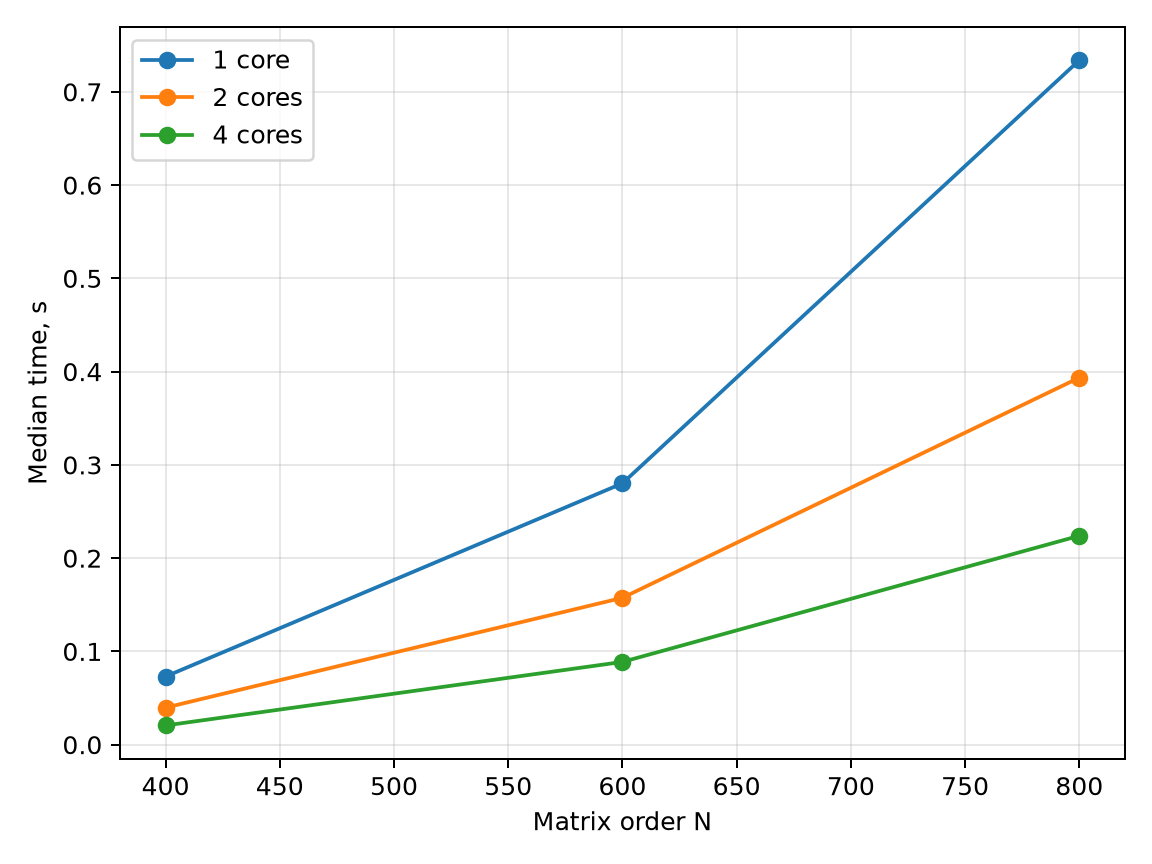
\includegraphics[width=.78\textwidth]{scaling-by-size.png}
\caption{Залежність часу від порядку матриць і кількості ядер}
\end{figure}

Для контролю фактичного використання процесорів під час окремого запуску
при $N=1000$ через однакові інтервали виміряно завантаження дозволених
логічних ЦП. На одному ядрі $CPU~0$ був завантажений майже на $100\%$.
Після застосування маски \texttt{0,2,4,6} одночасно працювали чотири різні
фізичні ядра (рис.~\ref{fig:cpu-load}).

\begin{figure}[H]\centering
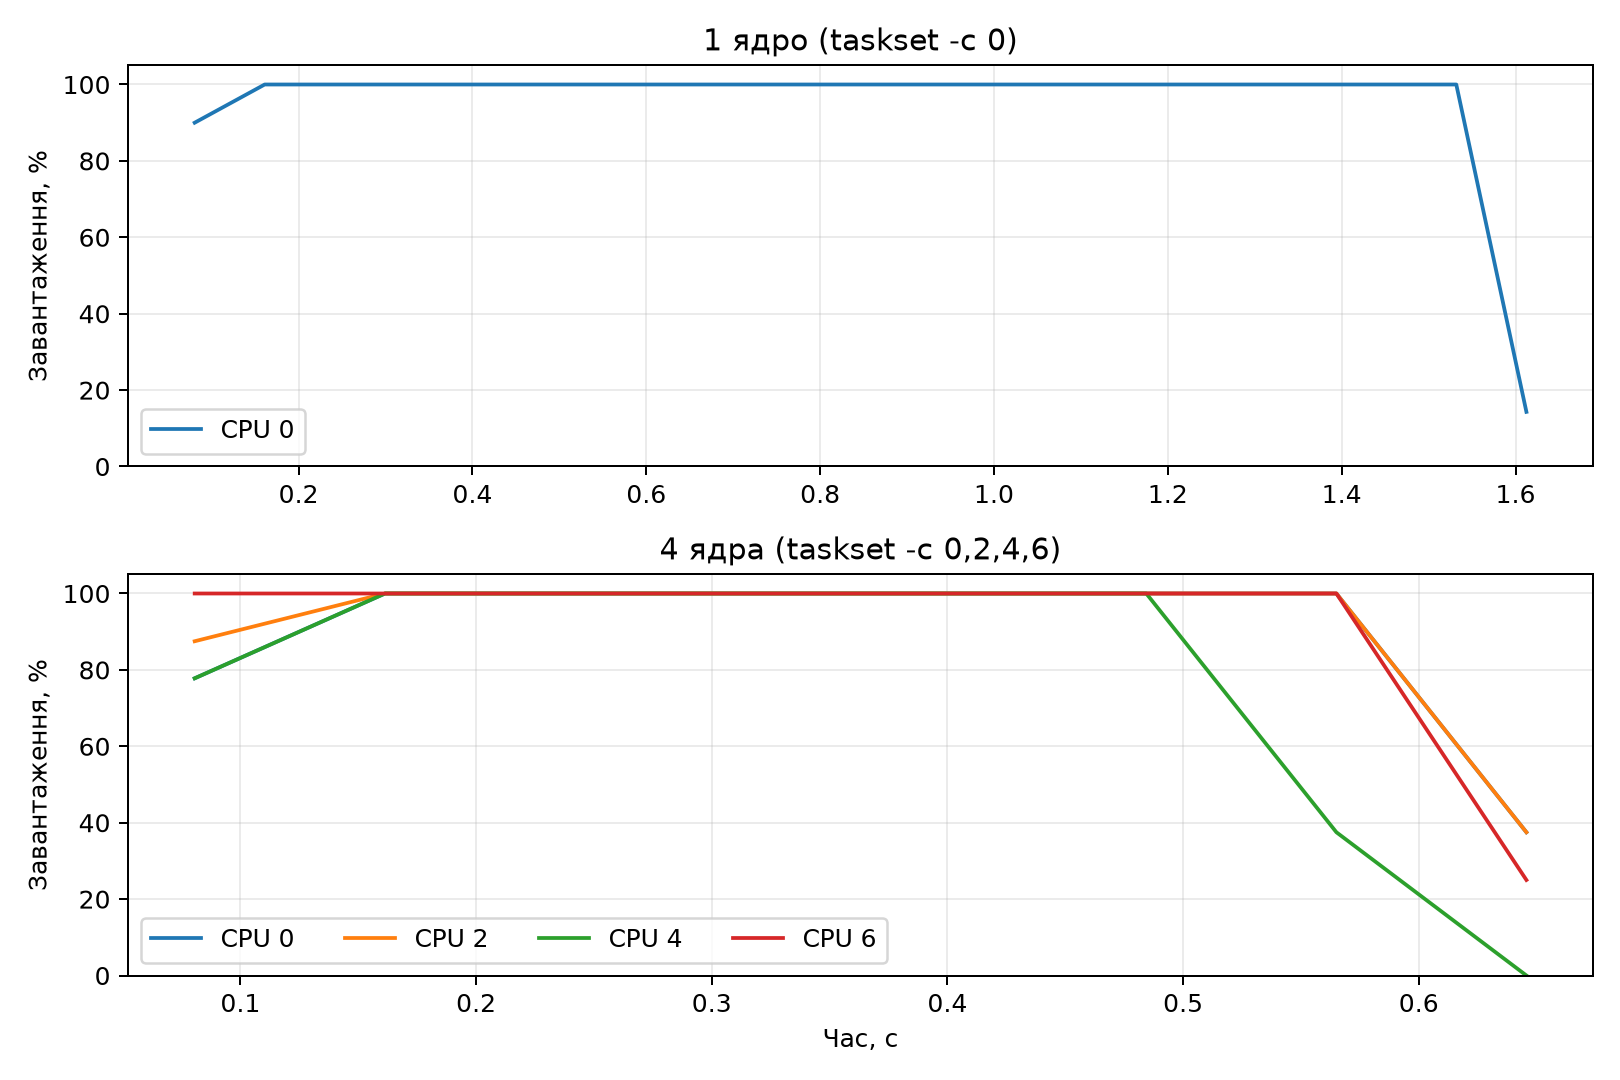
\includegraphics[width=.92\textwidth]{cpu-utilization.png}
\caption{Завантаження процесорів при запуску на одному та чотирьох ядрах}
\label{fig:cpu-load}
\end{figure}

Додатково стан процесора зафіксовано безпосередньо в установленому в
системі диспетчері ресурсів \texttt{btop 1.4.8}. Диспетчер отримує поточні
показники Linux із віртуальної файлової системи \texttt{/proc}. Знімки
вікна виконано штатним засобом композитора Wayland \texttt{niri}; сторонні
програми для моніторингу або створення знімків не встановлювалися.

На рис.~\ref{fig:btop-one} видно повне завантаження логічного процесора
$C0$, тоді як решта процесорів виконують лише фонові задачі системи. У
списку процесів зафіксовано виконання \texttt{lab4 1100}.
На рис.~\ref{fig:btop-four} процесори $C0$, $C2$, $C4$ та $C6$
одночасно мають завантаження близько $100\%$. Це підтверджує, що чотири
задачі OpenMP виконуються паралельно на чотирьох заданих фізичних ядрах.

\begin{landscape}
\begin{figure}[p]\centering
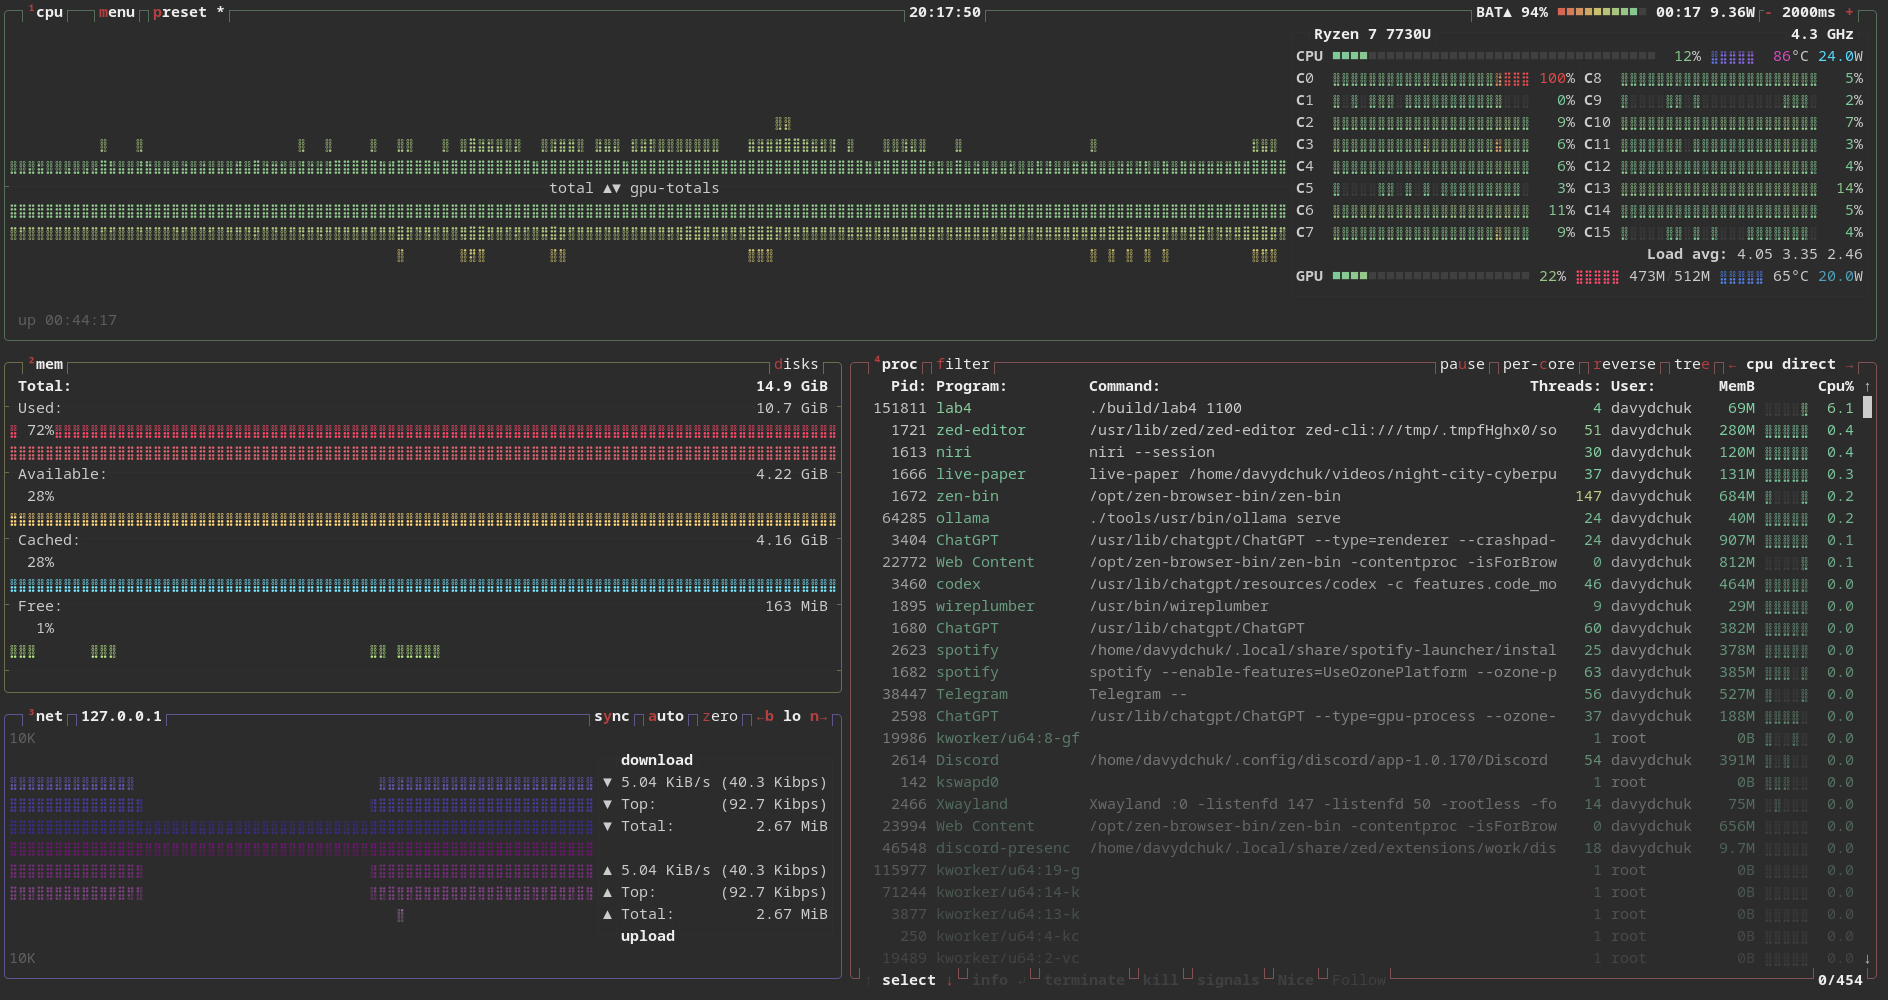
\includegraphics[width=.97\linewidth]{btop-1-core.png}
\caption{Системний монітор \texttt{btop}: виконання ЛР4 на одному ядрі
(маска \texttt{taskset -c 0})}
\label{fig:btop-one}
\end{figure}
\end{landscape}

\begin{landscape}
\begin{figure}[p]\centering
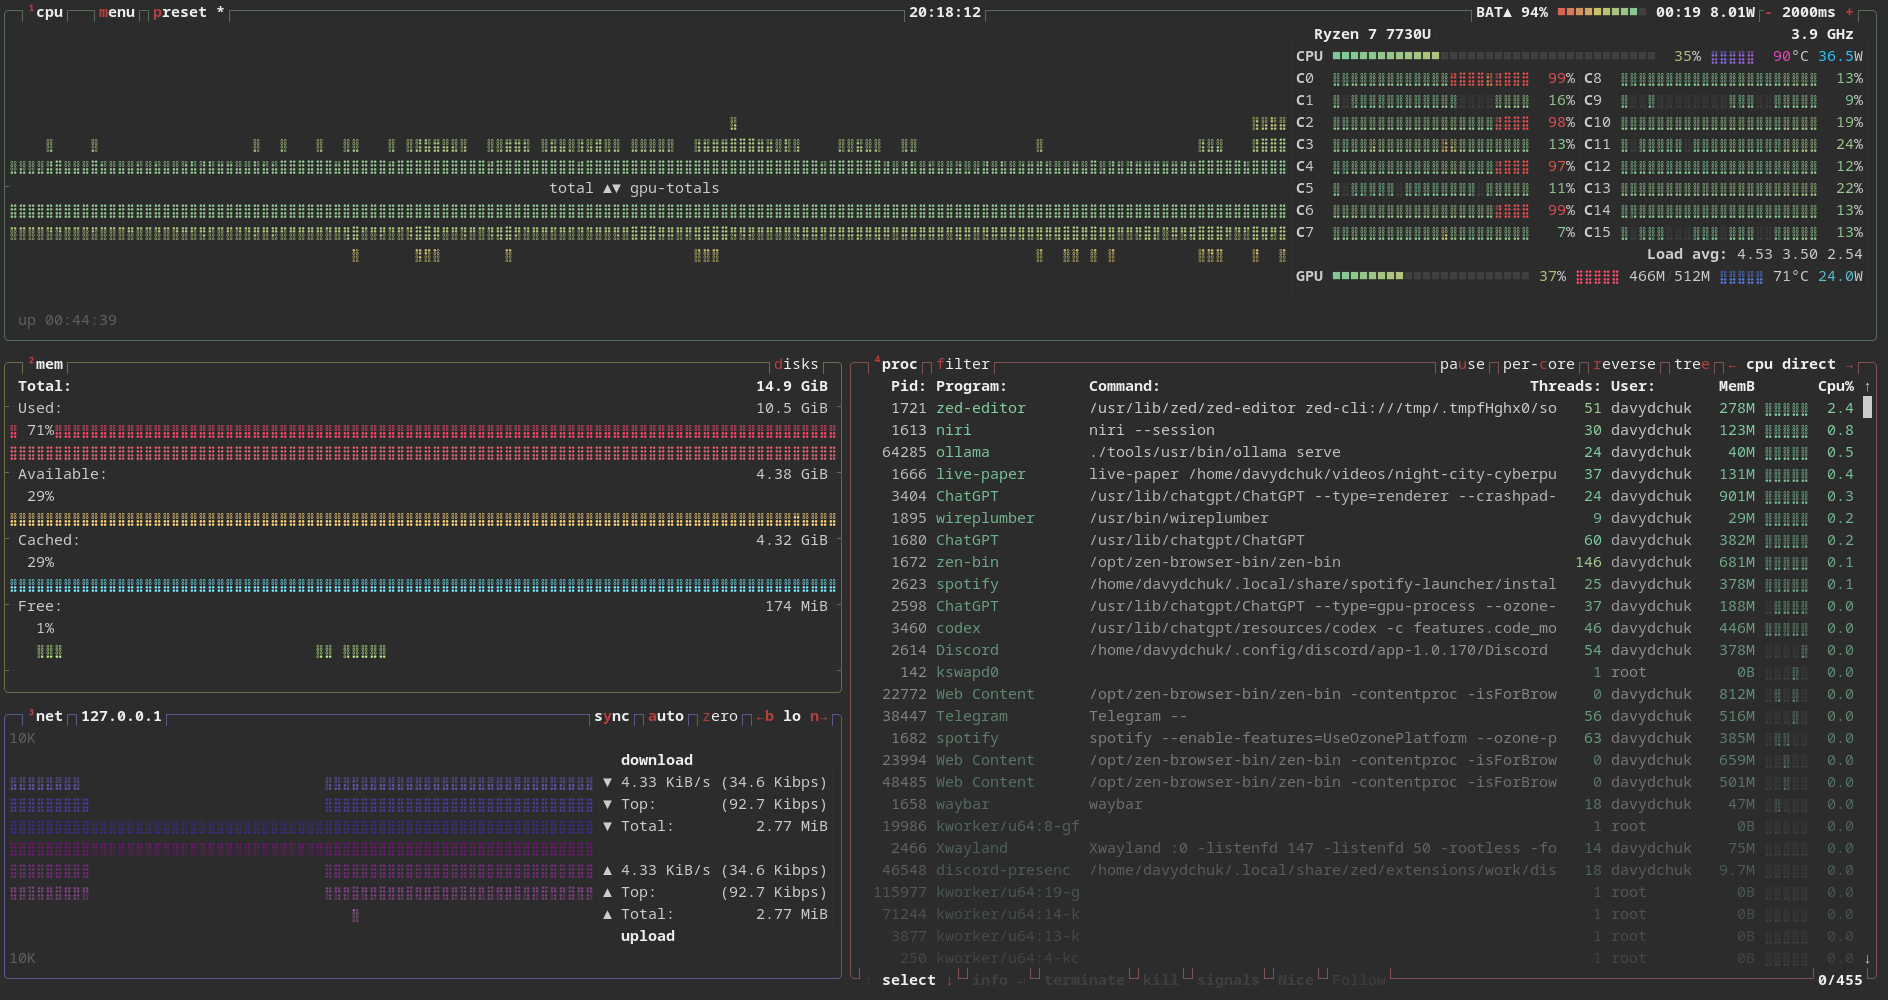
\includegraphics[width=.97\linewidth]{btop-4-cores.png}
\caption{Системний монітор \texttt{btop}: виконання ЛР4 на чотирьох ядрах
(маска \texttt{taskset -c 0,2,4,6})}
\label{fig:btop-four}
\end{figure}
\end{landscape}

\subsubsection*{Додаткове дослідження межі масштабування}
Основних OpenMP-потоків у програмі рівно чотири. Тому надання процесу понад
чотирьох ядер не створює додаткових виконавців. Це перевірено при $N=800$.

\begin{table}[H]\centering\renewcommand{\arraystretch}{1.15}
\begin{tabular}{|c|c|c|}\hline
\textbf{Доступні логічні ЦП}&$T_p$, с&$K_p$\\\hline
1&0,733879&1,000\\\hline
2&0,393534&1,865\\\hline
4&0,224002&3,276\\\hline
8&0,219795&3,339\\\hline
16&0,231963&3,164\\\hline
\end{tabular}
\caption{Додаткове дослідження при $N=800$}
\end{table}

\begin{figure}[H]\centering
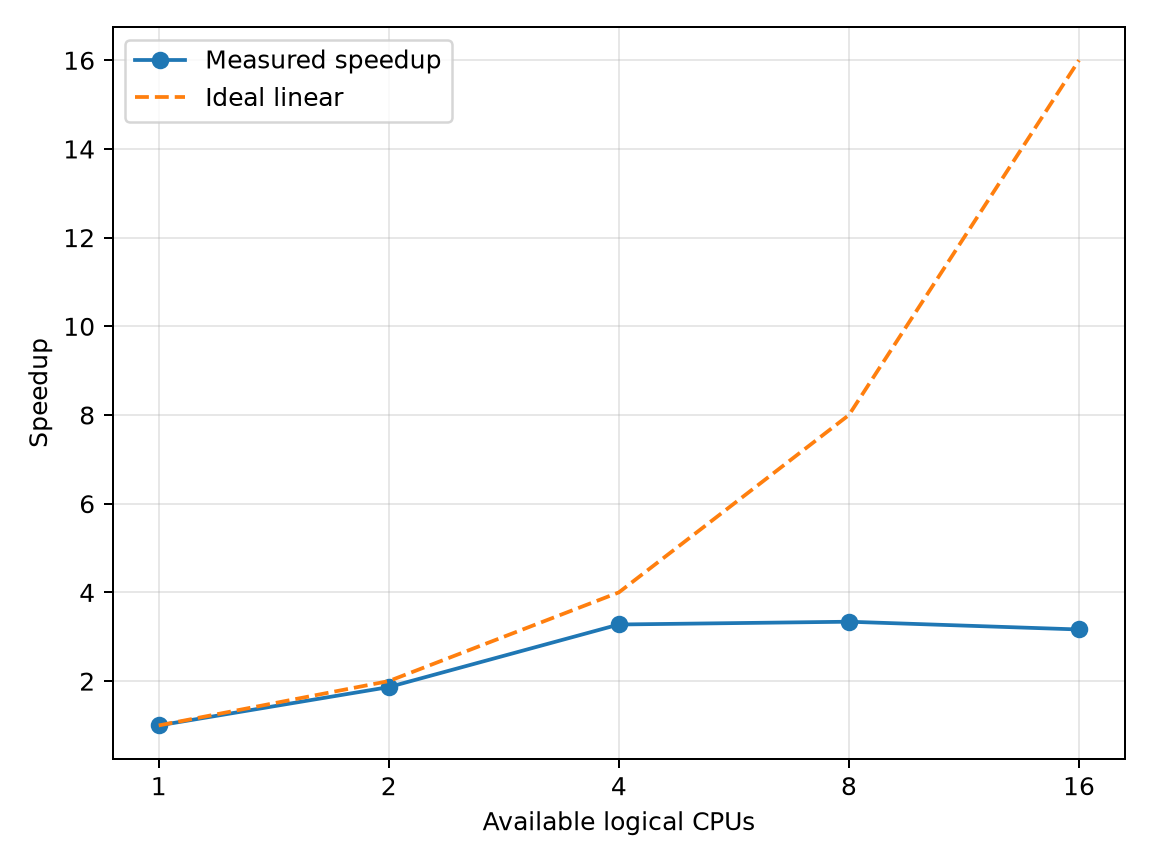
\includegraphics[width=.76\textwidth]{speedup-n800.png}
\caption{Виміряне та ідеальне прискорення при $N=800$}
\end{figure}

Після чотирьох ядер крива виходить на плато. Незначна різниця між 4, 8 і
16 доступними ЦП пояснюється плануванням ОС та зміною частоти процесора, а
не додатковим алгоритмічним паралелізмом. Контрольна сума в усіх запусках
при $N=800$ дорівнювала $410112000000$, тому зміна конфігурації не
вплинула на математичний результат.

\section{Висновки}
\begin{enumerate}[leftmargin=*,itemsep=.35em]
\item Розроблено паралельний математичний алгоритм варіанта 7. Обчислення
матриць розподілено за неперетинними стовпцями, а скалярний добуток --- за
частинами векторів.
\item Складено алгоритми $T_1$--$T_4$ із точками сигналізації й очікування,
трьома фазовими бар’єрами та критичними ділянками для спільних скалярів.
\item Побудовано структурну схему, яка відповідає алгоритмам і коду:
$B_1$ завершує введення, $B_2$ --- проміжні обчислення, $B_3$ --- формування
$MA$; взаємне виключення реалізують \texttt{atomic}, lock і critical.
\item Реалізовано програму C++17/OpenMP. Контрольні приклади при $N=4$ і
$N=5$ підтвердили формулу~\eqref{eq:control} та коректність нерівних
діапазонів.
\item Проведено експериментальне дослідження. При $N=800$ отримано
$K_4=3{,}276$ і $E_4=81{,}9\%$. Додатковий експеримент показав, що понад
чотири ядра не дають суттєвого прискорення, оскільки алгоритм створює
чотири основні задачі.
\end{enumerate}

\appendix
\section{Лістинг програми}
\subsection{Головний файл Lab4.cpp}
\inputminted{cpp}{../src/Lab4.cpp}
\subsection{Клас даних Data.h}
\inputminted{cpp}{../src/Data.h}
\subsection{Реалізація Data.cpp}
\inputminted{cpp}{../src/Data.cpp}
\subsection{Спільний алгоритм Worker.h}
\inputminted{cpp}{../src/Worker.h}
\subsection{Потік T1}
\inputminted{cpp}{../src/T1.h}
\subsection{Потік T2}
\inputminted{cpp}{../src/T2.h}
\subsection{Потік T3}
\inputminted{cpp}{../src/T3.h}
\subsection{Потік T4}
\inputminted{cpp}{../src/T4.h}
\subsection{CMakeLists.txt}
\inputminted{cmake}{../src/CMakeLists.txt}

\end{document}
